% Compilar desde esta carpeta con tectonic PDP-C1-BDLPSV.tex
% También puede usarse XeLaTeX (dos pasadas). Requiere Times New Roman instalada.
\documentclass[a4paper,10pt]{article}
\usepackage[spanish,es-tabla,es-noshorthands]{babel}
\usepackage{fontspec}
\setmainfont{Times New Roman}
\usepackage[a4paper,left=2.5cm,right=2.5cm,top=2.5cm,bottom=2cm]{geometry}
\usepackage{graphicx}
\usepackage{caption,multicol}
\usepackage{tikz}
\usetikzlibrary{arrows.meta}
\usepackage[hidelinks]{hyperref}
\hypersetup{
  pdftitle={Diseño e implementación de Buscaminas en Pharo},
  pdfauthor={Tomás Benchat, Tiago Gabriel Domínguez, Lautaro Leguizamón, Santiago Portillo, Mateo Salinas Jiménez y Lázaro Villagra},
  pdflang={es-AR}
}

\pagestyle{empty}
\raggedbottom
\raggedcolumns
\setlength{\emergencystretch}{1em}
\setlength{\parindent}{0pt}
\setlength{\parskip}{6bp}
\setlength{\abovecaptionskip}{5bp}
\setlength{\belowcaptionskip}{5bp}
\setlength{\intextsep}{9bp}
\setlength{\textfloatsep}{10bp}
\setlength{\columnsep}{8mm}
\setlength{\multicolsep}{4bp}
\setlength{\tabcolsep}{5bp}
\DeclareCaptionFont{tamanoLeyenda}{\fontsize{10bp}{12bp}\selectfont}
\captionsetup{font=tamanoLeyenda,labelfont=bf,labelsep=period,hypcap=false,justification=centering,singlelinecheck=false}
\captionsetup[figure]{name=Fig.}
\captionsetup[table]{name=Tabla,position=top}

\makeatletter
\renewcommand{\section}{\@startsection{section}{1}{0pt}
  {12bp}{3bp}{\normalfont\fontsize{10bp}{12bp}\selectfont\bfseries}}
\renewcommand{\subsection}{\@startsection{subsection}{2}{0pt}
  {8bp}{2bp}{\normalfont\fontsize{10bp}{12bp}\selectfont\bfseries}}
\renewcommand{\subsubsection}{\@startsection{subsubsection}{3}{0pt}
  {8bp}{2bp}{\normalfont\fontsize{10bp}{12bp}\selectfont\bfseries}}
\renewcommand{\@seccntformat}[1]{\csname the#1\endcsname.\enspace}
\makeatother
\newcommand{\autor}[2]{\raisebox{.48ex}{\fontsize{8bp}{9bp}\selectfont #1}\,#2}
\newcommand{\correo}[2]{\autor{#1}{\href{mailto:#2}{#2}}}
\newcommand{\entradaAPA}{\par\hangindent=1.27cm\hangafter=1\noindent}

\begin{document}
\fontsize{10bp}{12bp}\selectfont

\begin{center}
  {\fontsize{16bp}{19bp}\selectfont\bfseries Diseño e implementación de Buscaminas en Pharo\par}
  \vspace{5bp}
  {\fontsize{11bp}{14bp}\selectfont\bfseries
  \autor{a}{Tomás Benchat}\quad
  \autor{b}{Tiago Gabriel Domínguez}\quad
  \autor{c}{Lautaro Leguizamón}\\
  \autor{d}{Santiago Portillo}\quad
  \autor{e}{Mateo Salinas Jiménez}\quad
  \autor{f}{Lázaro Villagra}\par}
  \vspace{3bp}
  Universidad Tecnológica Nacional, Facultad Regional Resistencia\\
  Ingeniería en Sistemas de Información, Paradigmas de Programación, K2.1, Grupo 36\\
  {\fontsize{9bp}{12bp}\selectfont
  \correo{a}{tomasbenchat@gmail.com}\quad
  \correo{b}{tiagodo630@gmail.com}\quad
  \correo{c}{lautaromwateol@gmail.com}\\
  \correo{d}{porti.santiago@gmail.com}\quad
  \correo{e}{mateosalinasj@gmail.com}\quad
  \correo{f}{lazarovillagra9@gmail.com}\par}
\end{center}

\begin{center}
\begin{minipage}{0.82\textwidth}
\setlength{\parskip}{6bp}
\textbf{Resumen}\par
Se desarrolló un Buscaminas en Smalltalk con Pharo 14.0 como trabajo integrador de Programación Orientada a Objetos. El diseño distribuye las responsabilidades entre la interfaz, la partida y el tablero. Las celdas con y sin mina comparten una clase base que reúne sus operaciones comunes. Como variante de las reglas clásicas, la cantidad de vidas depende de la dificultad. El proyecto se realizó para poner en práctica los principios de la programación orientada a objetos mediante el desarrollo de un juego completo.
\end{minipage}
\end{center}

\begin{multicols}{2}

\section{Introducción}

El escenario asignado propone limpiar un tablero de Buscaminas a partir de pistas numéricas. Al descubrir una casilla segura, su número indica cuántas de las ocho posiciones vecinas contienen minas. En los bordes y las esquinas se cuentan solo las vecinas que existen. Al abrir una casilla segura con cero minas vecinas, se descubren también las vecinas sin bandera. El jugador puede señalar con banderas las posiciones donde sospecha que hay minas y gana al descubrir todas las casillas seguras.

Se eligió como variante un sistema de vidas por dificultad. Cada nivel también tiene un tamaño de tablero distinto. En fácil se juega en una grilla cuadrada de $9 \times 9$ y se pueden cometer hasta dos errores. En medio, la grilla es cuadrada, de $16 \times 16$, y se puede cometer un error. En difícil, el tablero es rectangular, de 16 filas por 30 columnas, y la primera mina causa la derrota.

\subsection{Motivaciones}

Se eligió un juego sencillo para entender cómo funciona la programación orientada a objetos al resolver un problema concreto. El Buscaminas permitió aplicar la abstracción, el encapsulamiento y la herencia (Joyanes Aguilar, 2008), y asignar responsabilidades claras a cada clase.

\subsection{Objetivo}

El objetivo fue desarrollar un juego completo y funcional en Smalltalk con Pharo, aplicando los conceptos de orientación a objetos al diseño de las clases y a la forma en que colaboran. También se buscó aprender a coordinar un equipo de seis integrantes, repartir tareas, revisar cambios e integrar aportes con Git, GitHub e Iceberg.

\section{Desarrollo}

\subsection{Prototipo en Python}

Primero se armó una versión sencilla del Buscaminas en Python (Fig.~\ref{fig:mock-tablero}). El prototipo permitió ver cómo se repartían las tareas. Las celdas guardaban su estado, el tablero resolvía la apertura y la interfaz enviaba las jugadas por coordenadas a la partida. Observar esa interacción ayudó a definir las responsabilidades de las clases antes de pasar a Smalltalk.

\begin{center}
\begin{minipage}{\columnwidth}
  \centering
  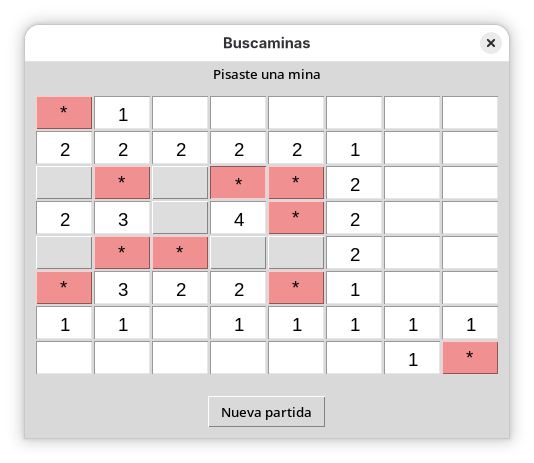
\includegraphics[width=0.73\linewidth]{assets/mock_tablero.png}
  \captionof{figure}{Tablero del prototipo en Python.}
  \label{fig:mock-tablero}
\end{minipage}
\end{center}

\subsection{Diseño del modelo}

Antes de implementar la versión en Smalltalk, se armó un diagrama de clases en draw.io para decidir qué responsabilidad tendría cada clase y cómo se comunicarían entre sí. La Fig.~\ref{fig:clases} muestra las relaciones principales del modelo implementado.

La interfaz se basa en Morphic (Aytar, 2002) y se ocupa de recibir los clics y dibujar el estado del juego. \texttt{Partida} coordina las jugadas, administra las vidas y las banderas, y decide cuándo se gana o se pierde. \texttt{Tablero} organiza la grilla, ubica las minas, calcula las pistas y abre las casillas en cascada.

\end{multicols}
\newpage

\begin{center}
\begin{minipage}{\textwidth}
  \centering
  \begin{tikzpicture}[
  x=1cm,y=1cm,
  clase/.style={
    draw,thin,fill=white,align=center,text width=3.55cm,inner sep=4.5pt,
    font=\fontsize{9bp}{10.5bp}\selectfont
  },
  etiqueta/.style={fill=white,inner sep=1.5pt,font=\fontsize{8.5bp}{10bp}\selectfont},
  asocia/.style={-{Latex[length=4pt,width=4pt]}},
  depende/.style={dashed,-{Latex[open,length=4pt,width=4pt]}},
  compone/.style={{Diamond[length=5.5pt,width=4pt]}-},
  agrega/.style={{Diamond[open,length=5.5pt,width=4pt]}-},
  hereda/.style={-{Triangle[open,length=5pt,width=6pt]}}
]
  \node[clase] (menu) at (2.0,0) {\textbf{MenuJuego}\\ \texttt{abrir}};
  \node[clase] (vista) at (7.75,0) {\textbf{TableroMorph}\\ \texttt{actualizar}};
  \node[clase] (casilla) at (13.5,0) {\textbf{CeldaMorph}\\ \texttt{mouseDown:}};
  \node[clase] (partida) at (7.75,-2.35) {\textbf{Partida}\\ \texttt{descubrirCelda:}\\ \texttt{alternarBandera:}};
  \node[clase] (reloj) at (2.0,-2.35) {\textbf{Reloj}\\ \texttt{iniciar}, \texttt{terminar}};
  \node[clase] (tablero) at (7.75,-4.45) {\textbf{Tablero}\\ \texttt{celdaEnFila:columna:}};
  \node[clase] (celda) at (7.75,-6.45) {\textit{abstracta}\\ \textbf{Celda}\\ \texttt{descubrir}, \texttt{tieneMina}};
  \node[clase] (conmina) at (4.7,-8.35) {\textbf{CeldaConMina}\\ \texttt{tieneMina} → \texttt{true}};
  \node[clase] (sinmina) at (10.8,-8.35) {\textbf{CeldaSinMina}\\ \texttt{tieneMina} → \texttt{false}};

  \draw[depende] (menu) -- node[etiqueta,above] {crea} (vista);
  \draw[compone] (vista) -- (casilla);
  \draw[asocia] (vista.south) -- (partida.north);
  \draw[asocia] (casilla.south) |- node[etiqueta,pos=.76,above] {envía jugadas} (partida.east);
  \draw[compone] (partida.west) -- (reloj.east);
  \draw[agrega] (partida.south) -- (tablero.north);
  \draw[compone] (tablero.south) -- node[etiqueta,right] {1..*} (celda.north);
  \draw[hereda] (conmina.north) |- ([xshift=-.65cm,yshift=-.48cm]celda.south) -- ([xshift=-.65cm]celda.south);
  \draw[hereda] (sinmina.north) |- ([xshift=.65cm,yshift=-.48cm]celda.south) -- ([xshift=.65cm]celda.south);
\end{tikzpicture}

  \captionof{figure}{Diagrama de clases del Buscaminas.}
  \label{fig:clases}
\end{minipage}
\end{center}

\begin{multicols}{2}

La cohesión se aprecia en que cada clase reúne operaciones relacionadas con su tarea. \texttt{Celda} guarda el estado de una casilla y \texttt{Reloj} mide el tiempo. \texttt{Partida} decide cuándo iniciar o detener el reloj y le pide al tablero que abra la casilla elegida. Así, la regla para descontar vidas queda en la partida, y el cálculo de las casillas vecinas queda en el tablero. El tablero puede construirse por separado y asociarse a una partida.

El ocultamiento de información es parcial. \texttt{Tablero} mantiene la matriz internamente y valida las coordenadas antes de devolver una celda. \texttt{TableroMorph} obtiene una referencia al tablero a través de \texttt{Partida}. Cada \texttt{CeldaMorph} consulta la celda lógica de su posición para dibujarla y envía las jugadas a \texttt{Partida}. Así, el modelo puede procesar jugadas sin abrir una ventana, aunque la vista conoce los objetos del modelo y su protocolo.

\subsection{Implementación}

El juego se desarrolló en Smalltalk con Pharo 14.0. Se usó Git para registrar los cambios, GitHub para compartir el repositorio e Iceberg para trabajar con el paquete desde Pharo. Las tareas se organizaron en un tablero Kanban con las columnas \emph{Pendiente}, \emph{En proceso} y \emph{Finalizado}. El equipo también coordinó por WhatsApp y revisó código en sesiones de Discord. El paquete se guardó en formato Tonel en \href{https://github.com/tomasben/pdp-tpi}{github.com/tomasben/pdp-tpi}.

El juego se inicia con \texttt{MenuJuego abrir} en el Playground de Pharo. Al elegir la dificultad en el menú (Fig.~\ref{fig:menu}), se crea una \texttt{Partida} mediante \texttt{nivel:}. La configuración asigna el tablero, las vidas y una bandera por mina.

\columnbreak

\texttt{TableroMorph} crea un \texttt{CeldaMorph} por posición y abre la ventana con el total de minas, las vidas y el reloj en cero.

\begin{center}
\begin{minipage}{\columnwidth}
  \centering
  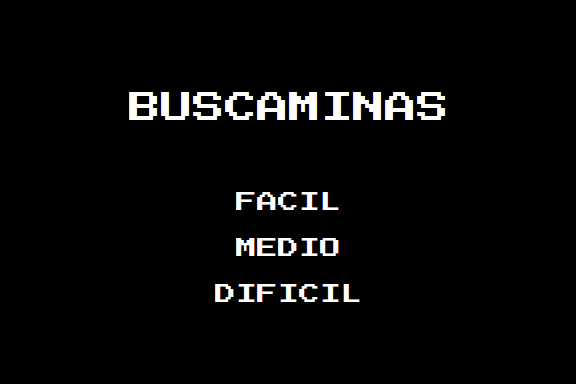
\includegraphics[width=0.78\linewidth]{assets/menu.png}
  \captionof{figure}{Menú de selección de dificultad.}
  \label{fig:menu}
\end{minipage}
\end{center}

Durante una partida activa, \texttt{CeldaMorph} obtiene del tablero la celda de su posición y le pasa ese objeto a \texttt{Partida}. El clic derecho alterna la bandera de una casilla oculta si quedan banderas disponibles o si ya estaba marcada. El izquierdo pide descubrirla. \texttt{Partida} ignora esa jugada si la casilla está marcada o descubierta, e inicia \texttt{Reloj} en el primer descubrimiento válido.

\texttt{Partida} le pide a \texttt{Tablero} que abra la posición. En la primera apertura, el tablero intenta dejar libre de minas la zona elegida. Si se abre una casilla segura con cero minas vecinas, la apertura se propaga a sus vecinas seguras y sin bandera. Después, \texttt{TableroMorph} actualiza el indicador de vidas y la representación de cada casilla. La Fig.~\ref{fig:secuencia} muestra ese intercambio en una jugada sobre una casilla segura.

\end{multicols}
\newpage

\begin{center}
\begin{minipage}{\textwidth}
  \centering
  \begin{tikzpicture}[
  x=1cm,y=1cm,
  clase/.style={
    draw,thin,fill=white,inner sep=5pt,minimum width=2.3cm,
    font=\fontsize{9.5bp}{11bp}\selectfont\bfseries
  },
  mensaje/.style={-{Latex[length=4pt,width=4pt]}},
  texto/.style={inner sep=2pt,fill=white,font=\fontsize{9bp}{10.5bp}\selectfont}
]
  \node[clase] (vista) at (1.45,0) {TableroMorph};
  \node[clase] (casilla) at (5.25,0) {CeldaMorph};
  \node[clase] (partida) at (9.0,0) {Partida};
  \node[clase] (tablero) at (14.35,0) {Tablero};

  \foreach \objeto in {vista,casilla,partida,tablero}
    \draw[dashed,black!55] (\objeto.south) -- (\objeto |- 0,-4.55);

  \draw[mensaje] (casilla |- 0,-.85) --
    node[texto,above] {\texttt{descubrirCelda:}} (partida |- 0,-.85);

  \draw[mensaje] (partida |- 0,-1.50) --
    node[texto,above] {\texttt{descubrirCeldaEnFila:columna:}} (tablero |- 0,-1.50);

  \draw[mensaje] (tablero |- 0,-2.08) -- ++(.8,0) -- ++(0,-.66) -- (tablero |- 0,-2.74);
  \node[texto,anchor=east,align=right] at (14.15,-2.41)
    {\texttt{descubrirCelda:} en cascada\\Omite las celdas ya abiertas o marcadas};

  \draw[mensaje] (casilla |- 0,-3.45) --
    node[texto,above] {\texttt{actualizar}} (vista |- 0,-3.45);

  \draw[mensaje] (vista |- 0,-4.15) --
    node[texto,above] {\texttt{actualizar} cada casilla} (casilla |- 0,-4.15);
\end{tikzpicture}

  \captionof{figure}{Secuencia de mensajes de una apertura en cascada.}
  \label{fig:secuencia}
\end{minipage}
\end{center}

\begin{multicols}{2}

Después de abrir la casilla, \texttt{Partida} vuelve a consultarla porque en la primera jugada el tablero puede haberse generado de nuevo. Si abrió una mina, descuenta una vida y la partida sigue mientras queden vidas. Si abrió una casilla segura, revisa si quedan otras por descubrir. Al ganar o perder, \texttt{Partida} registra el resultado y detiene el reloj. En caso de derrota, también le pide a \texttt{Tablero} que revele todas las minas (Fig.~\ref{fig:derrota}).

\begin{center}
\begin{minipage}{\columnwidth}
  \centering
  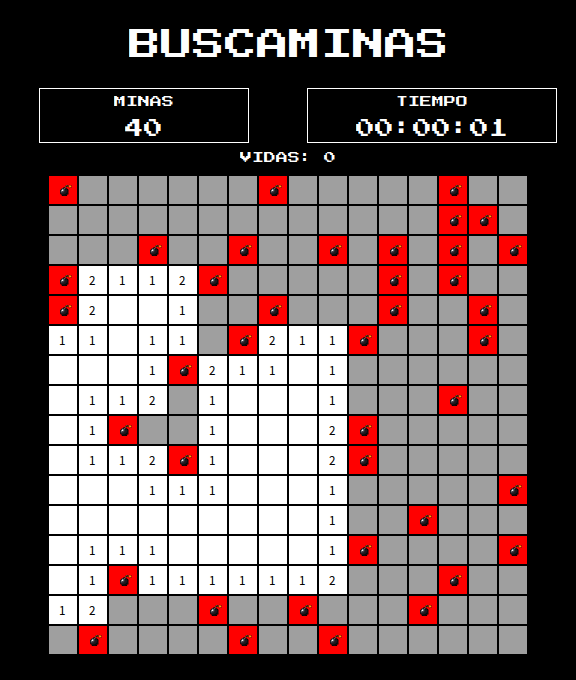
\includegraphics[width=0.85\linewidth]{assets/derrota.png}
  \captionof{figure}{Tablero de nivel medio con todas las minas reveladas.}
  \label{fig:derrota}
\end{minipage}
\end{center}

El tablero queda visible y la partida ya no acepta jugadas. Después de una derrota, un clic izquierdo sobre el tablero inicia la transición circular al menú. Los íconos de bomba y bandera y la tipografía de estilo arcade están incluidos en el paquete de Pharo.

\columnbreak

\subsection{Clases a detalle}

\begin{samepage}
\subsubsection{Celda}
\begingroup
\fontsize{8.5bp}{10.5bp}\selectfont
\setlength{\topsep}{3bp}
\setlength{\partopsep}{0pt}
\begin{verbatim}
Object << #Celda
    slots: { #fila . #columna .
             #estaDescubierta . #estaMarcada .
             #cantidadMinasVecinas };
    package: 'Buscaminas'
\end{verbatim}
\endgroup
\end{samepage}

Cada \texttt{Celda} representa una casilla del tablero. En el diseño inicial se pensó en usar una sola clase \texttt{Celda} con un atributo booleano para distinguir las casillas con mina de las casillas seguras. Luego se eligió representar esos dos tipos mediante \texttt{CeldaConMina} y \texttt{CeldaSinMina}, tal como se muestra en la Fig.~\ref{fig:clases}. Las dos heredan de \texttt{Celda}, que reúne las coordenadas, el estado de la casilla, la cantidad de minas vecinas y métodos comunes como \texttt{descubrir}, \texttt{marcar} y \texttt{desmarcar}. Así, esas operaciones se escriben una sola vez.

La clase base deja \texttt{tieneMina} como método abstracto mediante \texttt{subclassResponsibility}. En Pharo, este mensaje indica que las subclases deben redefinir el método (Ducasse et al., 2018). \texttt{CeldaConMina} lo redefine para devolver \texttt{true} y \texttt{CeldaSinMina} lo redefine para devolver \texttt{false}. La respuesta sigue siendo booleana, pero queda definida por la clase de la casilla.

\begin{samepage}
\subsubsection{Tablero}
\begingroup
\fontsize{8.5bp}{10.5bp}\selectfont
\setlength{\topsep}{3bp}
\setlength{\partopsep}{0pt}
\begin{verbatim}
Object << #Tablero
    slots: { #filas . #columnas .
             #celdas . #cantidadMinas };
    package: 'Buscaminas'
\end{verbatim}
\endgroup
\end{samepage}

\texttt{Tablero} representa la grilla rectangular y se encarga de distribuir las minas y calcular las pistas. \texttt{cantidadMinas:} genera la grilla y calcula cuántas minas rodean a cada casilla. Se guardó ese número en cada \texttt{Celda} para que la interfaz pueda leer la pista cuando la casilla queda visible. El mensaje \texttt{celdaEnFila:columna:} permite ubicar una casilla y valida que las coordenadas estén dentro de los límites.

\texttt{descubrirCeldaEnFila:columna:} recibe la posición que se quiere abrir. Si se abre una casilla segura con cero minas vecinas, \texttt{descubrirCelda:} se aplica a las vecinas seguras y deja intactas las marcadas. El tablero también informa cuántas casillas seguras quedan por abrir. Con ese dato, \texttt{Partida} decide si se ganó.

\begin{samepage}
\subsubsection{Partida}
\begingroup
\fontsize{8.5bp}{10.5bp}\selectfont
\setlength{\topsep}{3bp}
\setlength{\partopsep}{0pt}
\begin{verbatim}
Object << #Partida
    slots: { #tablero . #estado . #nivel .
             #banderasRestantes . #reloj .
             #vidasResantes };
    package: 'Buscaminas'
\end{verbatim}
\endgroup
\end{samepage}

\texttt{Partida} coordina el juego. Guarda el tablero, el nivel, el reloj, el estado de la partida y los contadores de vidas y banderas. \texttt{nivel:} crea la partida a partir de una configuración que reúne el tablero y las vidas de cada dificultad. Las reglas para descubrir y marcar casillas se concentran en \texttt{descubrirCelda:} y \texttt{alternarBandera:}, que verifican el estado de la partida antes de actuar.

La clase delega la apertura en \texttt{Tablero} y decide qué hacer con el resultado. Si aparece una mina, \texttt{perderVida} descuenta una vida. Si se descubren todas las casillas seguras o se agotan las vidas, \texttt{terminarConEstado:} registra el resultado y detiene el reloj. Esto permite mantener la decisión de cuándo termina el juego en un solo lugar.

\begin{samepage}
\subsubsection{Reloj}
\begingroup
\fontsize{8.5bp}{10.5bp}\selectfont
\setlength{\topsep}{3bp}
\setlength{\partopsep}{0pt}
\begin{verbatim}
Object << #Reloj
    slots: { #inicio . #acumulado . #estado };
    package: 'Buscaminas'
\end{verbatim}
\endgroup
\end{samepage}

\texttt{Reloj} representa el cronómetro de una partida. Guarda cuándo empezó el tramo actual, cuánto tiempo se acumuló antes y en qué estado está. \texttt{iniciar} empieza desde cero, \texttt{pausar} guarda el tiempo transcurrido y \texttt{reanudar} continúa desde ese valor. \texttt{terminar} deja fijo el tiempo final. Mientras el reloj corre, \texttt{tiempoTranscurrido} suma al acumulado la diferencia entre la hora actual y la de inicio.

En el flujo del juego, \texttt{Partida} inicia y detiene el reloj. \texttt{TableroMorph} consulta \texttt{tiempoFormateado} para mostrarlo en horas, minutos y segundos.

\subsection{Discusión y análisis}

Se buscó separar más la interfaz de las reglas del juego. En la versión actual, \texttt{Tablero} conserva la matriz de celdas y \texttt{Partida} da acceso al tablero. Cada \texttt{CeldaMorph} usa su fila y columna para obtener una celda del modelo. Después lee ese objeto para dibujarlo y se lo pasa a \texttt{Partida} al descubrir una casilla o alternar una bandera.

La idea era que la interfaz indicara cada jugada solo con la fila y la columna. La vista también necesitaba recibir el estado visible de cada casilla, como la bandera o el número de minas vecinas. No se llegó a definir cómo enviar esos datos y mantenerlos al día cuando una jugada modifica muchas casillas, como en una apertura en cascada. Queda como una mejora deseable porque permitiría actualizar el tablero visual sin que la interfaz acceda a las celdas del modelo.

Se consideró crear una clase \texttt{Jugador} para agrupar las vidas, las banderas disponibles y otros datos de quien juega. Se optó por gestionar esos datos en \texttt{Partida} para simplificar la implementación.

Una decisión central fue concentrar el final del juego en \texttt{Partida}. Con las vidas por dificultad, abrir una mina y perder la partida son eventos distintos. \texttt{Partida} descuenta la vida, \texttt{Tablero} revela las minas cuando se agotan y la interfaz se encarga de la transición visual.

En la primera apertura, el tablero se vuelve a generar hasta encontrar una casilla inicial libre de minas y de minas vecinas, con un límite de 1000 intentos. Si se alcanza ese límite, se usa la última grilla. Al regenerarla se pierden las marcas previas, pero el contador de banderas conserva su valor. Quedó pendiente preservar esas marcas y garantizar una primera casilla segura.

Durante las partidas se observó que el juego respondía más lento a medida que se acumulaban jugadas. La causa de esa lentitud quedó sin determinar y el problema no se resolvió.

\section{Conclusiones}

La división de responsabilidades permitió incorporar las vidas y el retorno al menú en componentes distintos. La jerarquía de celdas mostró cómo reutilizar operaciones comunes mediante la herencia. La pérdida de fluidez a medida que se acumulaban jugadas quedó pendiente de resolver.

El trabajo en equipo con un repositorio compartido permitió revisar los cambios de a uno y contrastar el diseño con el comportamiento del juego. El resultado es una implementación jugable que sirve para explicar cómo se traducen las reglas de un problema en objetos que colaboran entre sí.

\section*{Bibliografía}

\begingroup
\fontsize{8bp}{10bp}\selectfont
\raggedright
\entradaAPA Aytar, O. (2002). \textit{A guide to work with Squeak Morph classes}. Northeastern University.

\entradaAPA Ducasse, S., Chloupis, D., Hess, N., \& Zagidulin, D. (2018). \textit{Pharo by example 5}. Square Bracket Associates. \href{https://books.pharo.org/updated-pharo-by-example/pdf/2018-09-29-UpdatedPharoByExample.pdf}{books.pharo.org/\allowbreak updated-pharo-by-example/}

\entradaAPA Joyanes Aguilar, L. (2008). \textit{Fundamentos de programación: Algoritmos, estructura de datos y objetos} (4.ª ed.). McGraw-Hill Interamericana de España.

\par
\endgroup
\end{multicols}
\end{document}
